\documentclass[border=5pt, multi, tikz]{standalone}
\usetikzlibrary{quotes,arrows.meta}

\usepackage{xcolor}
\definecolor{morange}{RGB}{255,127,14}
\definecolor{mblue}{RGB}{31,119,180}
\definecolor{mred}{RGB}{214,39,40}
\definecolor{mpurple}{RGB}{148,103,189}
\definecolor{mgreen}{RGB}{44,160,44}

\begin{document}
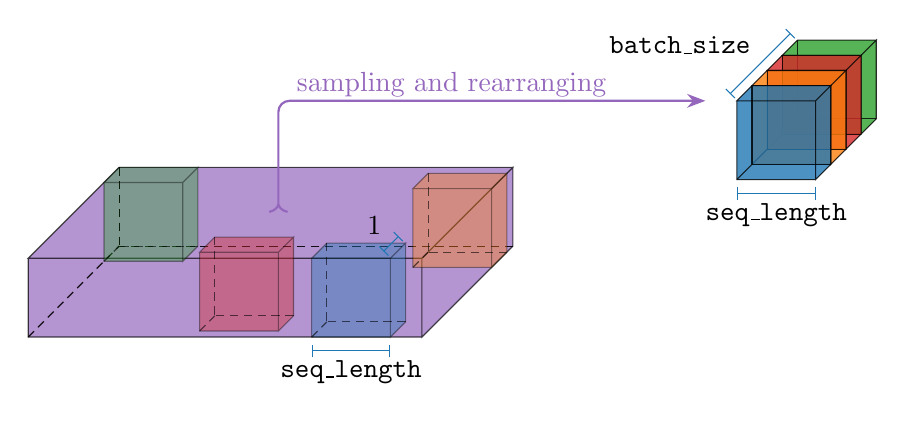
\begin{tikzpicture}[every edge quotes/.append style={auto, text=black}]
  \pgfmathsetmacro{\cubex}{5}
  \pgfmathsetmacro{\cubey}{1}
  \pgfmathsetmacro{\cubez}{3}
  \pgfmathsetmacro{\originx}{0}
  \pgfmathsetmacro{\originy}{0}
  \pgfmathsetmacro{\originz}{0}
  
  \draw [draw=black, every edge/.append style={draw=black, densely dashed, opacity=.9}, fill=mpurple, opacity=.7]
    (\originx,\originy,\originz) coordinate (o) -- ++(-\cubex,0,0) coordinate (a) -- ++(0,0-\cubey,0) coordinate (b) edge coordinate [pos=1] (g) ++(0,0,0-\cubez)  -- ++(\cubex,0,0) coordinate (c) -- cycle
    (o) -- ++(0,0,0-\cubez) coordinate (d) -- ++(0,0-\cubey,0) coordinate (e) edge (g) -- (c) -- cycle
    (o) -- (a) -- ++(0,0,0-\cubez) coordinate (f) edge (g) -- (d) -- cycle;
    ;

    \pgfmathsetmacro{\cubex}{1}
    \pgfmathsetmacro{\cubey}{1}
    \pgfmathsetmacro{\cubez}{.5}
    \pgfmathsetmacro{\originx}{-.4}
    \pgfmathsetmacro{\originy}{0}
    \pgfmathsetmacro{\originz}{0}
    
    \draw [draw=black, every edge/.append style={draw=black, densely dashed, opacity=.6}, fill=mblue, opacity=.4]
      (\originx,\originy,\originz) coordinate (o) -- ++(-\cubex,0,0) coordinate (a) -- ++(0,0-\cubey,0) coordinate (b) edge coordinate [pos=1] (g) ++(0,0,0-\cubez)  -- ++(\cubex,0,0) coordinate (c) -- cycle
      (o) -- ++(0,0,-\cubez) coordinate (d) -- ++(0,0-\cubey,0) coordinate (e) edge (g) -- (c) -- cycle
      (o) -- (a) -- ++(0,0,-\cubez) coordinate (f) edge (g) -- (d) -- cycle;
    \path [every edge/.append style={draw=mblue, |-|}]
      (b) +(0,-5pt) coordinate (b1) edge ["\texttt{seq\_length}"'] (b1 -| c)
      (o) +(-2.5pt,2.5pt) coordinate (f2) edge ["1"] ([xshift=-2.5pt,yshift=2.5pt]d)
      ;

      %\pgfmathsetmacro{\cubex}{1}
      %\pgfmathsetmacro{\cubey}{1}
      %\pgfmathsetmacro{\cubez}{.5}
      \pgfmathsetmacro{\originx}{0}
      \pgfmathsetmacro{\originy}{0}
      \pgfmathsetmacro{\originz}{-2.3}
      
      \draw [draw=black, every edge/.append style={draw=black, densely dashed, opacity=.6}, fill=morange, opacity=.4]
        (\originx,\originy,\originz) coordinate (o) -- ++(-\cubex,0,0) coordinate (a) -- ++(0,0-\cubey,0) coordinate (b) edge coordinate [pos=1] (g) ++(0,0,0-\cubez)  -- ++(\cubex,0,0) coordinate (c) -- cycle
        (o) -- ++(0,0,-\cubez) coordinate (d) -- ++(0,0-\cubey,0) coordinate (e) edge (g) -- (c) -- cycle
        (o) -- (a) -- ++(0,0,-\cubez) coordinate (f) edge (g) -- (d) -- cycle;
     ;

      %\pgfmathsetmacro{\cubex}{1}
      % \pgfmathsetmacro{\cubey}{1}
      % \pgfmathsetmacro{\cubez}{.5}
      \pgfmathsetmacro{\originx}{-1.9}
      \pgfmathsetmacro{\originy}{0}
      \pgfmathsetmacro{\originz}{-.2}
      
      \draw [draw=black, every edge/.append style={draw=black, densely dashed, opacity=.6}, fill=mred, opacity=.4]
        (\originx,\originy,\originz) coordinate (o1) -- ++(-\cubex,0,0) coordinate (a) -- ++(0,0-\cubey,0) coordinate (b) edge coordinate [pos=1] (g) ++(0,0,0-\cubez)  -- ++(\cubex,0,0) coordinate (c) -- cycle
        (o1) -- ++(0,0,-\cubez) coordinate (d) -- ++(0,0-\cubey,0) coordinate (e) edge (g) -- (c) -- cycle
        (o1) -- (a) -- ++(0,0,-\cubez) coordinate (f) edge (g) -- (d) -- cycle;
     ;

      %\pgfmathsetmacro{\cubex}{1}
      %\pgfmathsetmacro{\cubey}{1}
      %\pgfmathsetmacro{\cubez}{.5}
      \pgfmathsetmacro{\originx}{-4}
      \pgfmathsetmacro{\originy}{0}
      \pgfmathsetmacro{\originz}{-2.5}
      
      \draw [draw=black, every edge/.append style={draw=black, densely dashed, opacity=.6}, fill=mgreen, opacity=.4]
        (\originx,\originy,\originz) coordinate (o) -- ++(-\cubex,0,0) coordinate (a) -- ++(0,0-\cubey,0) coordinate (b) edge coordinate [pos=1] (g) ++(0,0,0-\cubez)  -- ++(\cubex,0,0) coordinate (c) -- cycle
        (o) -- ++(0,0,-\cubez) coordinate (d) -- ++(0,0-\cubey,0) coordinate (e) edge (g) -- (c) -- cycle
        (o) -- (a) -- ++(0,0,-\cubez) coordinate (f) edge (g) -- (d) -- cycle;
     ;

     %%%%%%%%%%%%%%%%%%%%%%%%%%%%%%%%%%%%%%%%%%%%%%%%%%%%%%%%%%%%%%%%%%%%%%
     % second part 

     \pgfmathsetmacro{\cubex}{1}
    \pgfmathsetmacro{\cubey}{1}
    \pgfmathsetmacro{\cubez}{.5}
    \pgfmathsetmacro{\originx}{5}
    \pgfmathsetmacro{\originy}{2}
    

      \pgfmathsetmacro{\originz}{-1.5}
      
      \draw [draw=black, fill=mgreen, opacity=.8]
        (\originx,\originy,\originz) coordinate (o) -- ++(-\cubex,0,0) coordinate (a) -- ++(0,0-\cubey,0) coordinate (b) edge coordinate [pos=1] (g) ++(0,0,0-\cubez)  -- ++(\cubex,0,0) coordinate (c) -- cycle
        (o) -- ++(0,0,-\cubez) coordinate (d) -- ++(0,0-\cubey,0) coordinate (e) edge (g) -- (c) -- cycle
        (o) -- (a) -- ++(0,0,-\cubez) coordinate (f1) edge (g) -- (d) -- cycle;
     ;

     \pgfmathsetmacro{\originz}{-1}
      
     \draw [draw=black, fill=mred, opacity=.8]
       (\originx,\originy,\originz) coordinate (o) -- ++(-\cubex,0,0) coordinate (a) -- ++(0,0-\cubey,0) coordinate (b) edge coordinate [pos=1] (g) ++(0,0,0-\cubez)  -- ++(\cubex,0,0) coordinate (c) -- cycle
       (o) -- ++(0,0,-\cubez) coordinate (d) -- ++(0,0-\cubey,0) coordinate (e) edge (g) -- (c) -- cycle
       (o) -- (a) -- ++(0,0,-\cubez) coordinate (f) edge (g) -- (d) -- cycle;
    ;



    \pgfmathsetmacro{\originz}{-.5}
      
    \draw [draw=black, fill=morange, opacity=.8]
      (\originx,\originy,\originz) coordinate (o) -- ++(-\cubex,0,0) coordinate (a) -- ++(0,0-\cubey,0) coordinate (b) edge coordinate [pos=1] (g) ++(0,0,0-\cubez)  -- ++(\cubex,0,0) coordinate (c) -- cycle
      (o) -- ++(0,0,-\cubez) coordinate (d) -- ++(0,0-\cubey,0) coordinate (e) edge (g) -- (c) -- cycle
      (o) -- (a) -- ++(0,0,-\cubez) coordinate (f) edge (g) -- (d) -- cycle;
   ;

      
   \pgfmathsetmacro{\originz}{0}
    
   \draw [draw=black, fill=mblue, opacity=.8]
     (\originx,\originy,\originz) coordinate (o2) -- ++(-\cubex,0,0) coordinate (a) -- ++(0,0-\cubey,0) coordinate (b) edge coordinate [pos=1] (g) ++(0,0,0-\cubez)  -- ++(\cubex,0,0) coordinate (c) -- cycle
     (o2) -- ++(0,0,-\cubez) coordinate (d) -- ++(0,0-\cubey,0) coordinate (e) edge (g) -- (c) -- cycle
     (o2) -- (a) -- ++(0,0,-\cubez) coordinate (f) edge (g) -- (d) -- cycle;
   \path [every edge/.append style={draw=mblue, |-|}]
     (b) +(0,-5pt) coordinate (b1) edge ["\texttt{seq\_length}"'] (b1 -| c)
     (a) +(-2.5pt,2.5pt) coordinate (f2) edge ["\texttt{batch\_size}"] ([xshift=-2.5pt,yshift=2.5pt]f1)
     ;

    \coordinate[above of=o1, yshift=-.5cm] (o3);
    \coordinate[left of=o2, xshift=-.4cm] (o4);
     \draw[>-Stealth,color=mpurple, rounded corners, thick] (o3) |- node  [text width=6cm, midway, xshift=2.2cm, yshift=.2cm, align=center] {sampling and rearranging} (o4);
\end{tikzpicture}
\end{document}